\chapter{Neural Ordinary Differential Equations}

In recent years Residual Networks (ResNet) \citep{he2016deep} have brought a great success in Deep Learning and especially in computer vision. They have proven to be effective against the vanishing and degradation gradient problems and have drastically eased the optimization of very deep neural networks. If we refer to the output vector of each layer as $ h_t $ where $ t $ stands for the layer, then Residual Networks can be mathematically described as:

\begin{displaymath}
    h_{t+1} = h_{t} + f(h_{t}; \ \theta_{t})
\end{displaymath}

where $ t \in \{0, ..., T\} $, $ h_t \in R^D $ and $ \theta_t $ being the parameters of the \emph{t}-th layer. These iterative updates can be seen as an Euler discretization of a continuous transformation \citep{lu2017beyond, haber2017stable, ruthotto2018deep}.

Moreover, as we add more layers and take smaller steps, in the limit, we parameterize the continuous dynamics of the hidden state using an ordinary differential equation (ODE) \textcolor{red}{vo abbreviations ODE} specified by a neural network:

\begin{equation}
    \label{odes}
    \frac{d h(t)}{d t} = f(h(t), \ t; \ \theta )
\end{equation}

\citet{chen2018neural} introduced this as a new family of deep neural network models, where the neural network outputs the gradient of the hidden state with respect to the depth. Then, given an initial state and the differential equation parameterized by the neural network, the final state is obtained by solving an ODE. The analogy they make is the one that considers this family of models to be the continuous case of ResNets. They call this family of models \emph{Neural ODEs}.

\begin{figure}[ht]
      \centering
      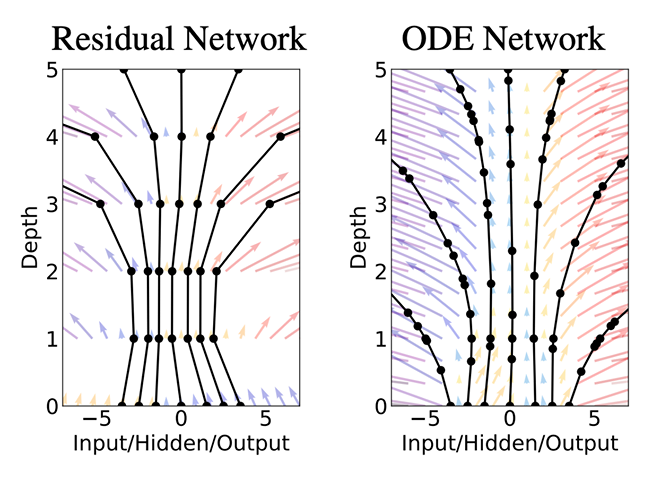
\includegraphics[width=0.7\columnwidth]{figures/resnet_vs_odes.png}
    %   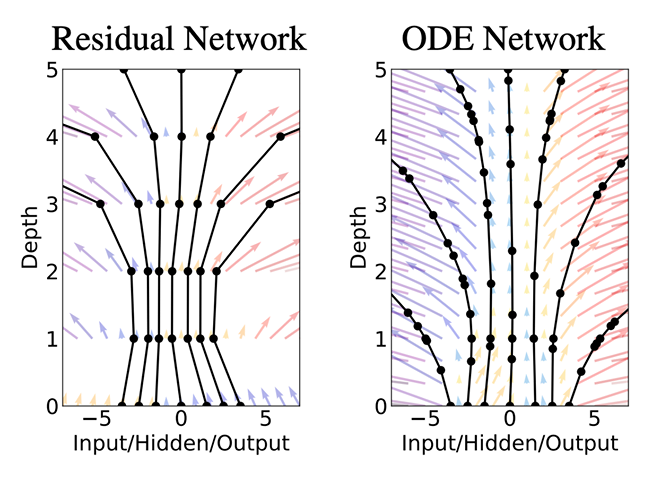
\includegraphics[width=0.5em]{figures/resnet_vs_odes.png}
      \caption{\emph{Left}: A Residual network defines a discrete sequence of finite transformations. \emph{Right}: A ODE network defines a vector that continuously transforms the state \citep{chen2018neural}.}
      \label{ode:resnet_vs_ode}
\end{figure}

In equation \ref{odes}, $ h(t) $ is the hidden state in the \emph{t}-th layer, and $ f $ is the neural network parameterized with $ \theta $. $ f $ takes $ h(t) $ and $ t $ as input and outputs the gradient of $ h(t) $ with respect to $ t $. Essentially, $ f $ is learning a vector field, which is why Neural ODEs can potentially be seen as models with infinite amount of layers. More precisely, the amount of layers is dynamically decided and delegated to the ODE solver.

Speaking of the ODE solver. 